\documentclass[a4paper, amsfonts, amssymb, amsmath, reprint, showkeys, nofootinbib, twoside]{revtex4-1}
\usepackage[english]{babel}
\usepackage[utf8]{inputenc}
\usepackage[colorinlistoftodos, color=green!40, prependcaption]{todonotes}
\usepackage[pdftex, pdftitle={Article}, pdfauthor={Author}]{hyperref}
\usepackage{amsthm}
\usepackage{mathtools}
\usepackage{physics}
\usepackage{xcolor}
\usepackage{caption}
\usepackage{hyperref}
\usepackage{multirow}
\usepackage{amsmath}
\usepackage{amssymb}
\usepackage{graphicx}
\graphicspath{Images}
\usepackage[left=23mm,right=13mm,top=35mm,columnsep=15pt]{geometry} 
\usepackage{adjustbox}
\usepackage{placeins}
\usepackage[T1]{fontenc}
\usepackage{float}
%\usepackage{longtable}
\usepackage{csquotes}
\usepackage{refstyle}
\usepackage{lipsum}

\begin{document}

\title{Study of Hall effect and Magnetoresistance in Bismuth}
\author{Swaroop Ramakant Avarsekar}
\email{swaroop.avarsekar@niser.ac.in}
\affiliation{School of Physical Sciences, National Institute of Science Education and Research, HBNI, Jatni -752050, India}
\date{\today}
	
\begin{abstract}
In this experiment, we study the magnetoresistance of Bismuth and also find the Hall coefficient of the sample. The increase in magnetoresistance is observed with increase in applied magnetic field. With two different probe current, we calculate the Hall coefficient of Bi. The Hall coefficient at probe current 190 mA is $(4.58\pm0.09) \times10^{-7} m^3/C$. and at 150 mA is $(4.19\pm0.08) \times10^{-7} m^3/C$, with average being $(4.38\pm0.12) \times10^{-7} m^3/C$. 
\end{abstract}
	
\keywords{Hall effect, Magnetoresistance, Gaussmeter}
	
\maketitle

\section{Theory}
\subsection{Hall Effect}
Hall effect is a phenomenon when a current carrying conductor/crystal where the direction of current is along x, with direction of magnetic field H from top gives the voltage across the ends 1 and 2 due to Hall effect, as shown in Figure(1). This magnetic field exerts a Lorentz force on charge carriers as given below:
\begin{equation}
	\bar{F}=e(\bar{v}\times\bar{H})
\end{equation}

where e is charge of electron, v is drift velocity of charge carriers, H is magnetic field applied. This Lorentz force drags the electrons and holes towards opposite ends of the crystal, resulting a electric field, called Hall field ($E_H$), opposite to Lorentz force. Deflection of charge carriers takes place until Hall field cancels the Lorentz Force giving rise to a potential difference, called Hall voltage ($V_H$) . 

\begin{figure}[H]
	\centering
	\includegraphics[scale=0.36]{1} 
	\caption{Hall effect in a crystal}
	\label{1}
\end{figure}

The field along y-axis is given by 
\begin{equation}
	E_m=vH=\mu E_x H
\end{equation}

This electric field is related to current density and conductivity as
\begin{equation}
	\sigma E_x=J_x
\end{equation}

The Hall coefficient $R_H$ is defined as 
\begin{equation}
	R_H=E_m/J_x H=\mu E_x /J_x=\mu/\sigma=1/ne
\end{equation}

The Hall voltage is proportional to 1/n and $ \mu =R_H \sigma $. Experimentally, the Hall coefficient is given by 
\begin{equation}
	R_H=\frac{V_y /b}{(I_x/bt)H}=V_y t/I_x H
\end{equation}

where b and t are width and thickness of the sample.

If voltage across the input is kept constant, then Hall angle as the ratio of applied and measured voltages.
\begin{equation}
	\phi=V_y/V_x=E_m b/E_x I=\mu b H/l 
\end{equation}

where l is the length of the crystal. 

\subsection{Magnetoresistance}
Magnetoresistance is property of a material where resistivity changes with the magnetic field applied. This phenomena was discovered by Lord Kelvin. It is due to fact that the drift velocity of all charge carriers is not same. When magnetic field is applied, the Hall voltage compensates Lorentz force, with slower carriers being over compensated and faster ones with under compensated resulting in reduced mean free path, more collisions and increased resistivity. 

Three cases of magnetoresistance depending on the structure of the electron orbitals at the Fermi surface In metals with closed Fermi surfaces, the electrons are constrained to their orbit in k-space and the effect of the magnetic field is to increase the cyclotron frequency of the electron in its closed orbit. For metals with equal numbers of electrons and holes, the magnetoresistance increases with
H up to the highest fields measured and is independent of crystallographic orientation. Bismuth falls in this class. Metals that contain Fermi surfaces with open orbits in some crystallographic directions will exhibit large magnetoresistance for fields applied in those directions, whereas the resistance will saturate in other directions, where the orbits are closed

\section{Experiment \& Analysis}
\begin{figure}[H]
	\centering
	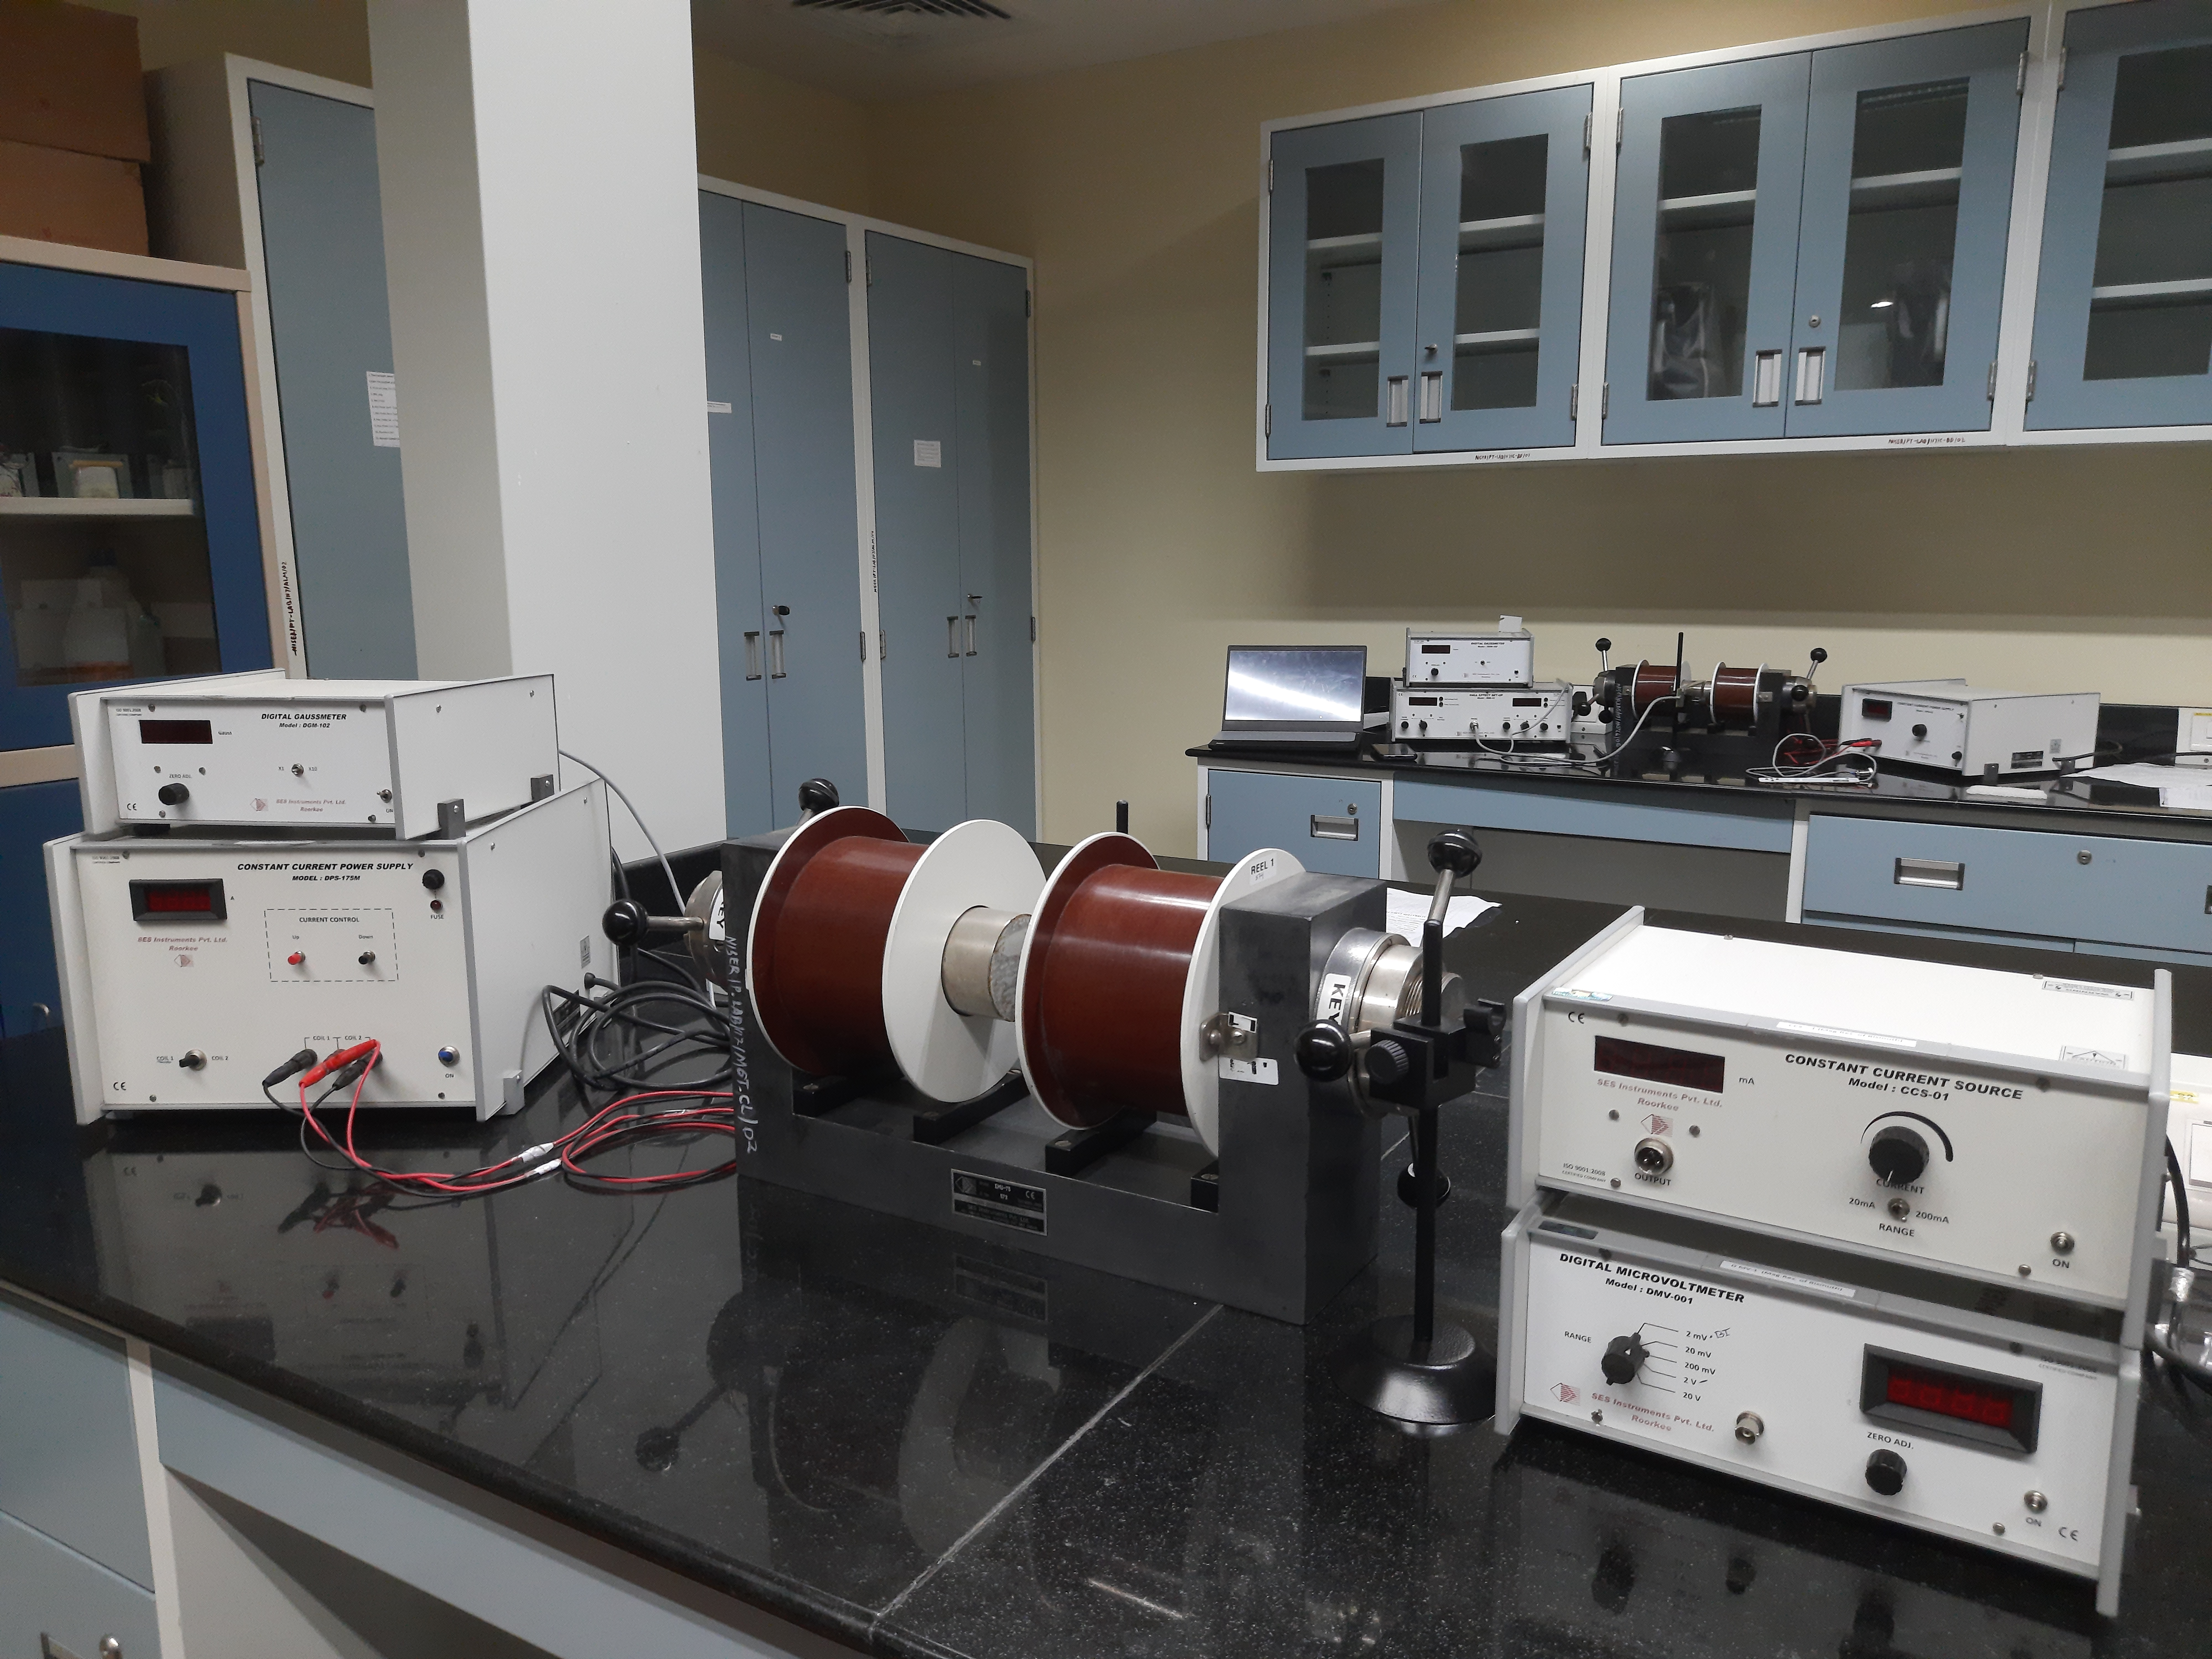
\includegraphics[scale=0.03]{2} 
	\caption{Experimental setup in laboratory}
	\label{2}
\end{figure}
Magnetoresistance, Four probes, and Hall probes with Bi sample and constant current source and power supply. Gaussmeter to measure magnetic fields. Electromagnets , microvoltmeter and multipurpose stand will be required for this experiment. The setup is shown in Figure (2).

\begin{table}[H]
	\centering
	\caption{Magnetoresistance Table for probe current 190 mA}
	\label{t1}
	\resizebox{\columnwidth}{!}{%
		\begin{tabular}{|c|c|c|c|c|c|}
			\hline
			Magnetic field (G) & Hall Voltage (mV) & $R_{m} (\Omega)$ & $\Delta R$/R & Log (H) & Log ($\Delta R/R$) \\ \hline
			0    & 0.301 & 0.00158 & 0.0000 &             &               \\ \hline
			594  & 0.303 & 0.00159 & 0.0093 & 2.773786445 & -2.030252657  \\ \hline
			858  & 0.304 & 0.00160 & 0.0127 & 2.933487288 & -1.897627091  \\ \hline
			1223 & 0.304 & 0.00160 & 0.0127 & 3.087426457 & -1.897627091  \\ \hline
			1557 & 0.305 & 0.00161 & 0.0160 & 3.192288613 & -1.796169451  \\ \hline
			1932 & 0.308 & 0.00162 & 0.0260 & 3.286007122 & -1.585316085  \\ \hline
			2340 & 0.31  & 0.00163 & 0.0326 & 3.369215857 & -1.486184612  \\ \hline
			2740 & 0.311 & 0.00164 & 0.0360 & 3.437750563 & -1.443986932  \\ \hline
			3020 & 0.314 & 0.00165 & 0.0460 & 3.480006943 & -1.337531602  \\ \hline
			3330 & 0.316 & 0.00166 & 0.0526 & 3.522444234 & -1.278753601  \\ \hline
			3690 & 0.32  & 0.00168 & 0.0660 & 3.567026366 & -1.180745498  \\ \hline
			3990 & 0.321 & 0.00169 & 0.0693 & 3.600972896 & -1.159347353  \\ \hline
			4280 & 0.321 & 0.00169 & 0.0693 & 3.631443769 & -1.159347353  \\ \hline
			4610 & 0.322 & 0.00169 & 0.0726 & 3.663700925 & -1.138954194  \\ \hline
			4870 & 0.327 & 0.00172 & 0.0893 & 3.687528961 & -1.049275894  \\ \hline
			5050 & 0.326 & 0.00172 & 0.0859 & 3.703291378 & -1.065790982  \\ \hline
			5330 & 0.327 & 0.00172 & 0.0893 & 3.726727209 & -1.049275894  \\ \hline
			5550 & 0.33  & 0.00174 & 0.0993 & 3.744292983 & -1.003194424  \\ \hline
			5740 & 0.331 & 0.00174 & 0.1026 & 3.758911892 & -0.9888599714 \\ \hline
			5970 & 0.333 & 0.00175 & 0.1093 & 3.775974331 & -0.9615368442 \\ \hline
			6090 & 0.334 & 0.00176 & 0.1126 & 3.784617293 & -0.9484939876 \\ \hline
			6130 & 0.335 & 0.00176 & 0.1159 & 3.787460475 & -0.935831444  \\ \hline
		\end{tabular}%
	}
\end{table}

\begin{table}[H]
	\centering
	\caption{Magnetoresistance Table for probe current 150 mA}
	\label{t2}
	\resizebox{\columnwidth}{!}{%
		\begin{tabular}{|c|c|c|c|c|c|}
			\hline
			Magnetic field (G) & Hall Voltage (mV) & $R_{m} (\Omega)$ & $\Delta R$/R & Log (H) & Log ($\Delta R/R$) \\ \hline
			0    & 0.222 & 0.00148 &        &             &               \\ \hline
			861  & 0.224 & 0.00149 & 0.0090 & 2.935003151 & -2.045322979  \\ \hline
			1143 & 0.224 & 0.00149 & 0.0090 & 3.05804623  & -2.045322979  \\ \hline
			1497 & 0.225 & 0.00150 & 0.0135 & 3.1752218   & -1.86923172   \\ \hline
			1785 & 0.228 & 0.00152 & 0.0270 & 3.25163822  & -1.568201724  \\ \hline
			2100 & 0.228 & 0.00152 & 0.0270 & 3.322219295 & -1.568201724  \\ \hline
			2360 & 0.229 & 0.00153 & 0.0315 & 3.372912003 & -1.501254934  \\ \hline
			2590 & 0.231 & 0.00154 & 0.0405 & 3.413299764 & -1.392110465  \\ \hline
			2850 & 0.232 & 0.00155 & 0.0450 & 3.45484486  & -1.346352974  \\ \hline
			3110 & 0.233 & 0.00155 & 0.0495 & 3.492760389 & -1.304960289  \\ \hline
			3330 & 0.235 & 0.00157 & 0.0586 & 3.522444234 & -1.232409622  \\ \hline
			3610 & 0.236 & 0.00157 & 0.0631 & 3.557507202 & -1.200224939  \\ \hline
			3860 & 0.238 & 0.00159 & 0.0721 & 3.586587305 & -1.142232992  \\ \hline
			4130 & 0.24  & 0.00160 & 0.0811 & 3.615950052 & -1.091080469  \\ \hline
			4340 & 0.241 & 0.00161 & 0.0856 & 3.63748973  & -1.067599373  \\ \hline
			4640 & 0.242 & 0.00161 & 0.0901 & 3.666517981 & -1.045322979  \\ \hline
			4920 & 0.244 & 0.00163 & 0.0991 & 3.691965103 & -1.003930294  \\ \hline
			5120 & 0.245 & 0.00163 & 0.1036 & 3.709269961 & -0.9846251384 \\ \hline
			5380 & 0.246 & 0.00164 & 0.1081 & 3.730782276 & -0.9661417327 \\ \hline
			5620 & 0.248 & 0.00165 & 0.1171 & 3.749736316 & -0.9313796265 \\ \hline
			5800 & 0.25  & 0.00167 & 0.1261 & 3.763427994 & -0.8991949431 \\ \hline
			6110 & 0.251 & 0.00167 & 0.1306 & 3.78604121  & -0.8839549766 \\ \hline
		\end{tabular}%
	}
\end{table}

\begin{table}[H]
	\centering
	\caption{Table for Hall effect }
	\label{t3}
	\resizebox{\columnwidth}{!}{%
		\begin{tabular}{|cc|cc|}
			\hline
			\multicolumn{2}{|c|}{Probe current=190mA}                    & \multicolumn{2}{c|}{Probe current=150 mA}                   \\ \hline
			\multicolumn{1}{|c|}{Magnetic field (G)} & Hall Voltage (mV) & \multicolumn{1}{c|}{Magnetic field (G)} & Hall Voltage (mV) \\ \hline
			\multicolumn{1}{|c|}{0}    & 0      & \multicolumn{1}{c|}{0}    & 0      \\ \hline
			\multicolumn{1}{|c|}{799}  & -0.008 & \multicolumn{1}{c|}{1168} & -0.006 \\ \hline
			\multicolumn{1}{|c|}{1145} & -0.01  & \multicolumn{1}{c|}{1432} & -0.008 \\ \hline
			\multicolumn{1}{|c|}{1325} & -0.012 & \multicolumn{1}{c|}{1760} & -0.01  \\ \hline
			\multicolumn{1}{|c|}{1427} & -0.013 & \multicolumn{1}{c|}{1877} & -0.011 \\ \hline
			\multicolumn{1}{|c|}{1647} & -0.015 & \multicolumn{1}{c|}{1950} & -0.011 \\ \hline
			\multicolumn{1}{|c|}{1824} & -0.017 & \multicolumn{1}{c|}{2230} & -0.013 \\ \hline
			\multicolumn{1}{|c|}{1960} & -0.018 & \multicolumn{1}{c|}{2490} & -0.015 \\ \hline
			\multicolumn{1}{|c|}{2140} & -0.019 & \multicolumn{1}{c|}{2730} & -0.015 \\ \hline
			\multicolumn{1}{|c|}{2290} & -0.02  & \multicolumn{1}{c|}{2980} & -0.017 \\ \hline
			\multicolumn{1}{|c|}{2500} & -0.022 & \multicolumn{1}{c|}{3300} & -0.018 \\ \hline
			\multicolumn{1}{|c|}{2730} & -0.023 & \multicolumn{1}{c|}{3580} & -0.02  \\ \hline
			\multicolumn{1}{|c|}{2960} & -0.026 & \multicolumn{1}{c|}{3830} & -0.021 \\ \hline
			\multicolumn{1}{|c|}{3160} & -0.027 & \multicolumn{1}{c|}{4050} & -0.022 \\ \hline
			\multicolumn{1}{|c|}{3300} & -0.028 & \multicolumn{1}{c|}{4260} & -0.025 \\ \hline
			\multicolumn{1}{|c|}{3530} & -0.03  & \multicolumn{1}{c|}{4460} & -0.026 \\ \hline
			\multicolumn{1}{|c|}{3720} & -0.031 & \multicolumn{1}{c|}{4830} & -0.027 \\ \hline
			\multicolumn{1}{|c|}{3890} & -0.032 & \multicolumn{1}{c|}{5120} & -0.028 \\ \hline
			\multicolumn{1}{|c|}{4020} & -0.033 & \multicolumn{1}{c|}{5510} & -0.029 \\ \hline
			\multicolumn{1}{|c|}{4210} & -0.034 & \multicolumn{1}{c|}{5650} & -0.03  \\ \hline
			\multicolumn{1}{|c|}{4420} & -0.036 & \multicolumn{1}{c|}{5910} & -0.031 \\ \hline
			\multicolumn{1}{|c|}{4720} & -0.038 & \multicolumn{1}{c|}{6050} & -0.032 \\ \hline
			\multicolumn{1}{|c|}{4930} & -0.04  & \multicolumn{1}{c|}{6130} & -0.032 \\ \hline
			\multicolumn{1}{|c|}{5150}               & -0.041            & \multicolumn{2}{c|}{\multirow{6}{*}{}}                      \\ \cline{1-2}
			\multicolumn{1}{|c|}{5310} & -0.042 & \multicolumn{2}{c|}{}              \\ \cline{1-2}
			\multicolumn{1}{|c|}{5500} & -0.042 & \multicolumn{2}{c|}{}              \\ \cline{1-2}
			\multicolumn{1}{|c|}{5670} & -0.043 & \multicolumn{2}{c|}{}              \\ \cline{1-2}
			\multicolumn{1}{|c|}{5880} & -0.043 & \multicolumn{2}{c|}{}              \\ \cline{1-2}
			\multicolumn{1}{|c|}{6070} & -0.044 & \multicolumn{2}{c|}{}              \\ \hline
		\end{tabular}%
	}
\end{table}

\subsection{Hall effect}

To find the Hall coefficient of Bi, we plot Magnetic field versus Hall voltage for two different probe current as shown in Figure (3) and (4).

\begin{figure}[H]
	\centering
	\includegraphics[scale=0.5]{3} 
	\caption{Hall voltage versus Magnetic field, I=190 mA}
	\label{2}
\end{figure}

\begin{figure}[H]
	\centering
	\includegraphics[scale=0.5]{4} 
	\caption{Hall voltage versus Magnetic field, I=150 mA}
	\label{2}
\end{figure}

We know that from equation (5) and figures (3) and (4), Slope is V/H with t and I being known quantities. t is the thickness of the sample, t= 1.2 mm.

Therefore,
\begin{equation}
	R_H=Slope.t/I
\end{equation}

Hall coefficient from probe current=190 mA is,
\begin{equation}
	R_H=-0.0726\times0.0012/190=4.58\times10^{-7} m^3/C
\end{equation}
 
 Hall coefficient from probe current=150 mA is,
 \begin{equation}
 	R_H=-0.0524\times0.0012/150=4.19\times10^{-7} m^3/C
 \end{equation}

Error in $R_H$ is:
\begin{equation}
	\Delta R_H=R_H\times\Delta Slope/Slope
\end{equation}

For probe current at 190 mA, we have
\begin{equation}
	\Delta R_H=4.58\times10^{-7} \frac{0.0015}{0.0726}=0.09\times10^{-7} m^3/C
\end{equation}

For probe current at 190 mA, we have
\begin{equation}
	\Delta R_H=4.19\times10^{-7} \frac{0.001}{0.0524}=0.08\times10^{-7} m^3/C
\end{equation}

The average Hall coefficient is $4.38 \times10^{-7} m^3/C$

Error in average value is $\sqrt{(0.08)^2+(0.09)^2}=0.12 \times10^{-7} m^3/C$

Therefore, average value of  Hall coefficient of Bismuth is $(4.38\pm0.12) \times10^{-7} m^3/C$

\subsection{Magnetoresistance}
\begin{figure}[H]
	\centering
	\includegraphics[scale=0.4]{9} 
	\caption{Plot for magnetoresistance for 190 mA of current}
	\label{2}
\end{figure}

\begin{figure}[H]
	\centering
	\includegraphics[scale=0.4]{10} 
	\caption{Plot for magnetoresistance for 150 mA of current}
	\label{2}
\end{figure}

\begin{figure}[H]
	\centering
	\includegraphics[scale=0.4]{ln1} 
	\caption{Plot for log(H) versus log($\Delta R$) for 190 mA}
	\label{2}
\end{figure}

\begin{figure}[H]
	\centering
	\includegraphics[scale=0.4]{ln2} 
	\caption{Plot for log(H) versus log($\Delta R$) for 150 mA}
	\label{2}
\end{figure}

\begin{figure}[H]
	\centering
	\includegraphics[scale=0.4]{kk} 
	\caption{Magnetoresistance dependence for different current}
	\label{2}
\end{figure}

It is observed from the figures (5), (6), (7), (8) and (9), that magnetoresistance of Bismuth linearly increases with the magnetic field applied. We supplied the probe current with 190 mA and 150 mA and magnetoresistance is studied. It is also seen that with higher probe current magnetoresistance increases, where the curve for 190 mA is seen higher than 150 mA.

\section{Conclusion}
In this experiment we studied the properties of Bi, which is semi-metal. Hall coefficient and Magnetoresistance at different probe current was studied.  The Hall coefficient of Bismuth at probe current 190 mA is $(4.58\pm0.09) \times10^{-7} m^3/C$. and at 150 mA is $(4.19\pm0.08) \times10^{-7} m^3/C$, with average being $(4.38\pm0.12) \times10^{-7} m^3/C$. It is expected that Hall coefficient should not change with different probe current, but here it arises due to Nernst effect, irregular power supply, heating, etc. Current through the probe should not be excess. It was also seen that magnetoresistance increases with increase in magnetic field in a linear fashion. Much of the error to this experiment have been contributed by the instruments used, some random errors may have crept into the data. 

\section{References}
\begin{enumerate}
\item{SPS NISER Lab Manual}
\item {\url{https://en.wikipedia.org/wiki/Hall_effect}}

\end{enumerate}

\end{document}